\documentclass[sigconf,nonacm]{acmart}

\usepackage{booktabs}
\usepackage{amsmath}
\usepackage{graphicx}

\settopmatter{printacmref=false}
\setcopyright{none}
\renewcommand\footnotetextcopyrightpermission[1]{}

\begin{document}

\title{The Accuracy Illusion: How Overlapping Samples Manufacture
Confidence, Not Skill, in Intraday Index Forecasting}

\author{Rachit Ranka}
\affiliation{%
  \institution{Department of Computer Science Engineering, Chandigarh University}
  \city{Mohali}
  \country{India}}
\email{rankarachit5@gmail.com}

\author{Aaditya Saini}
\affiliation{%
  \institution{Department of Computer Science Engineering, Chandigarh University}
  \city{Mohali}
  \country{India}}
\email{aadityasaini899@gmail.com}

\begin{abstract}
Intraday forecasting systems routinely report directional hit-rates between
60\% and 85\%, and those figures move real capital. We show they are not valid
estimates of skill. A $k$-bar-ahead forecast issued every bar shares $k{-}1$ of
its $k$ outcome bars with its neighbour; when the model's calls also persist, as
they do on a live system we instrument, the reported hit-rate acquires a
variance far larger than its nominal sample size implies. The reading is not
biased upward. Its stated precision is. A forecaster with \emph{exactly zero
skill}, simulated against real NSE index bars, posts a $\geq$71\% session once
in 50 while reporting an interval $1.66\times$ too narrow, rising to
$3.11\times$ at the per-minute density these systems publish.

We give the closed form behind this, the classical design effect with clusters
given by runs of identical calls, and a calibrated interval built on it that
covers at 96\% where the conventional one covers at 75\%. Applied to our own
results it leaves nothing: across 48 model--index--horizon tests, 16 clear
$p<0.05$ scored per bar and \emph{zero} clear it per event or at an effective
sample size. A premium-selling strategy we had published as this project's one
measurable edge fails the same correction. Break-even accuracy derived from
measured move distributions is 71.5\% at thirty minutes against a best achieved
51.2\%, and at five minutes no accuracy suffices under a symmetric bracket. Code
and raw results are public.
\end{abstract}

\ccsdesc[500]{Mathematics of computing~Time series analysis}
\ccsdesc[500]{Computing methodologies~Supervised learning by classification}
\ccsdesc[300]{Applied computing~Economics}
\ccsdesc[300]{Mathematics of computing~Hypothesis testing and confidence interval computation}

\keywords{overlapping observations, backtest overfitting, directional
forecasting, negative results, reproducibility, index derivatives}

\maketitle

\section{Introduction}

A system reporting 71\% directional accuracy is, on its face, extraordinary.
Work that controls for scoring unit, costs and multiple testing places realistic
out-of-sample intraday index accuracy close to a coinflip
\cite{timmermann2004,sullivan1999}, while surveys of the applied literature
catalogue many higher figures reported without those controls \cite{sezer2020}.

This paper began as an attempt to build such a system. Over fourteen months we
ran a live multi-horizon forecasting platform for Indian index derivatives, and
it reported 71\%. That number was wrong. The specific session producing it
cannot be re-audited, because the portion of the log holding it was lost before
this analysis; every figure below comes from sessions that survive.

The econometrics of overlapping observations is not new
\cite{hansen1980,richardson1991}. Boudoukh et al.\ \cite{boudoukh2008} show that
overlap manufactures apparent long-horizon predictability which vanishes under
correct inference. What that literature does not document is the magnitude of
the distortion in a now-ubiquitous practice: the every-minute multi-horizon
dashboard, where overlap meets a second ingredient, prediction persistence, and
is then amplified across a panel.

\textbf{Contributions.} (i) We measure the artefact as it occurs, showing that
overlap alone changes nothing and that inflation requires overlap \emph{and}
persistent predictions, with persistence calibrated from a production log.
(ii) We derive the effective sample size of such a stream, show it is governed
by $\mathbb{E}[L^2]/\mathbb{E}[L]$ over run lengths, and calibrate an interval
that covers at its nominal rate. (iii) We apply it to our own results and to a
complete control set --- shuffled labels, injected positive controls, nine
architectures, a block-bootstrap null --- and report that nothing survives.
(iv) We invert accuracy into a required-versus-achieved framing that shows the
gap is not close. Code, raw results and the free-data corpus are at
\url{https://github.com/rachitranka25/accuracy-illusion}.

\section{Related Work}

Hansen and Hodrick \cite{hansen1980} and Richardson and Smith
\cite{richardson1991} characterise inference under overlapping returns; Newey
and West \cite{newey1987} give the standard correction. That work concerns
regression coefficients. We apply the same logic to what practitioners publish,
the session hit-rate, and the correction we reach is the classical design effect
\cite{kish1965,moulton1990} with clusters given by runs of identical calls. The
contribution is its application to forecast streams, not the statistic.

On multiplicity, Harvey et al.\ \cite{harvey2016} argue the conventional $t>2$
threshold is indefensible after decades of factor mining. Bailey and López de
Prado \cite{bailey2014} introduce the Deflated Sharpe Ratio and Bailey et al.\
\cite{bailey2017} the Probability of Backtest Overfitting; White's Reality Check
\cite{white2000}, its refinement by Hansen \cite{hansen2005} and
Benjamini--Hochberg \cite{bh1995} provide complementary controls. Sullivan et
al.\ \cite{sullivan1999} apply the Reality Check to a universe of trading rules,
the direct precedent for our strategy sweep.

On machine learning for finance, Fischer and Krauss \cite{fischer2018} and
Krauss et al.\ \cite{krauss2017} report headline performance gross of costs; Gu
et al.\ \cite{gu2020} give a comprehensive comparison with modest out-of-sample
$R^2$. Zhang et al.\ \cite{zhang2019} and Kolm et al.\ \cite{kolm2023}
demonstrate genuine short-horizon alpha, both from message-level exchange data
rather than bars --- the distinction that matters here.

\begin{table*}[t]
\caption{Methodological comparison with representative prior work. ``Scoring
unit'' is the unit in which hit-rate or return is aggregated; per-bar scoring of
a multi-bar horizon is the condition under which the artefact of
Section~\ref{sec:mech} appears. MT: multiple-testing correction. NC: null
control (shuffled labels or equivalent). C: transaction costs modelled. R: code
and raw results public.}
\label{tab:related}
\small
\begin{tabular}{@{}llllcccc@{}}
\toprule
\textbf{Study} & \textbf{Market} & \textbf{Data granularity} &
\textbf{Scoring unit} & \textbf{MT} & \textbf{NC} & \textbf{C} & \textbf{R} \\
\midrule
Fischer \& Krauss \cite{fischer2018} & S\&P 500 & Daily bars & Per day, non-overlapping & --- & --- & pre-cost & --- \\
Krauss et al. \cite{krauss2017} & S\&P 500 & Daily bars & Per day, non-overlapping & --- & --- & pre-cost & --- \\
Gu et al. \cite{gu2020} & US equities & Monthly & Per month & partial & --- & partial & partial \\
Zhang et al. \cite{zhang2019} & LSE & Message-level LOB & Per event & --- & --- & --- & partial \\
Kolm et al. \cite{kolm2023} & Nasdaq & Message-level LOB & Per horizon & --- & --- & discussed & --- \\
\midrule
\textbf{This work} & NSE index & 5-min bars, EOD chains & \textbf{Per event ($k$-bar)} &
\checkmark & \checkmark & \checkmark & \checkmark \\
\bottomrule
\end{tabular}
\vspace{2pt}

\footnotesize MT here means Bonferroni and Benjamini--Hochberg, which applied
cleanly, plus the Deflated Sharpe Ratio and PBO/CSCV, which we ran and found
inapplicable and degenerate respectively (Section~\ref{sec:pred}). NC means
shuffled-label controls on every model plus injected positive controls. C means
explicit round-trip costs, inverted into a required-accuracy threshold. We omit
a row for ``typical applied studies'': characterising that population would
require citing specific papers as negative examples, and the argument does not
need it.
\end{table*}

\section{Data and Method}

All data is obtainable free from a retail brokerage account and public exchange
archives (Table~\ref{tab:data}). Three practical observations. Index spot prints
zero volume, so a feature computed as a ``VWAP'' on spot is an unweighted
expanding mean; real volume exists only on futures. The exchange's \emph{live}
option-chain API is geo-restricted while its static end-of-day archive is not,
which turned an assumed constraint into a decade of data. And brokers
authenticating by locally computed TOTP permit collection from any jurisdiction,
where SMS-based flows do not.

\begin{table}[t]
\caption{Free-data corpus. All collectors are public.}
\label{tab:data}
\small
\begin{tabular}{@{}llr@{}}
\toprule
\textbf{Asset} & \textbf{Period} & \textbf{Size} \\
\midrule
BANKNIFTY 5-min bars & 2025-02 -- 2026-07 & 26\,265 \\
NIFTY 50 5-min bars & 2025-02 -- 2026-07 & 26\,267 \\
3 further indices, 5-min & 2025 -- 2026 & 9.6k--14k \\
Option chain EOD + OI & 2024-07 -- 2026-07 & 1\,382\,738 \\
Long-history option chain & 2016-05 -- 2026-05 & 2\,181 d \\
Participant-wise OI & 2024-07 -- 2026-07 & 515 d \\
Index futures (real volume) & 2024-01 -- 2026-07 & 639 d \\
\bottomrule
\end{tabular}
\end{table}

Every accuracy passes through one harness. Splits are expanding-window
walk-forward with the $k$ bars whose labels overlap the test window purged from
training \cite{prado2018}. Accuracies carry Clopper--Pearson \cite{clopper1934}
intervals, exact binomial $p$-values and the Pesaran--Timmermann statistic
\cite{pt1992}, which is the appropriate null for directional accuracy. Every
model is additionally trained on randomly permuted labels; if real and shuffled
scores coincide, the pipeline is reading noise. A synthetic feature of known
strength is injected as a positive control, since a pipeline that cannot recover
planted signal cannot be trusted to report a null. Strategy returns use
non-overlapping $k$-bar holds with explicit costs.

\textbf{Units.} All analysis is on 5-minute bars, so the 30-minute horizon is
$k=6$ and a session yields $n=69$ forecasts. The production system emits a
forecast every \emph{minute}; pooled across indices its run lengths average 13.5
minutes (3.0 bars) with a longest of 207 minutes (41 bars).

\section{The Mechanism}
\label{sec:mech}

\subsection{Overlap is arithmetic}

Figure~\ref{fig:acf} shows the autocorrelation of the $k$-bar forward return two
ways. On overlapping windows it reaches 0.841 at lag 1 and decays to
approximately zero at \emph{exactly} lag $k$; sampled so no two observations
share a bar it is 0.067 and indistinguishable from zero thereafter. The pattern
reproduces at $k=6$ and $k=12$, with the decay landing on lag 6 and lag 12. The
correlation is a property of the sampling scheme, not the market.

\begin{figure}[t]
\centering
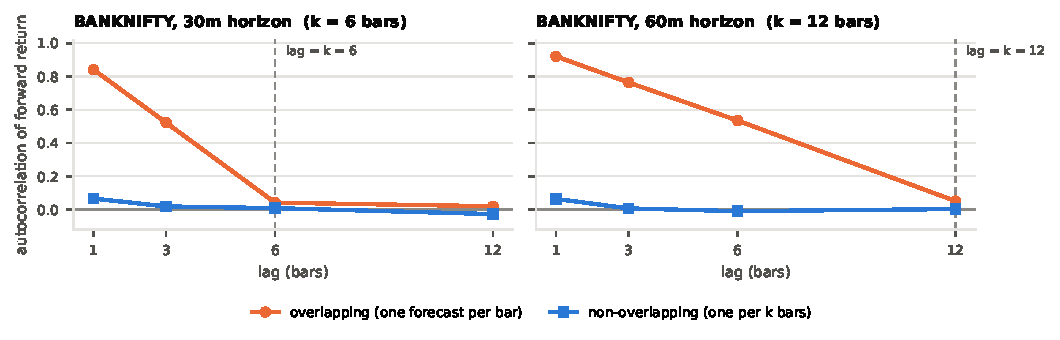
\includegraphics[width=\columnwidth]{figures/fig1_autocorrelation.pdf}
\caption{Forward-return autocorrelation, overlapping versus non-overlapping, at
two horizons. The overlapping series dies at exactly lag $k$ in both panels.}
\label{fig:acf}
\end{figure}

\subsection{Persistence is the second ingredient}

Overlap alone is insufficient. If predictions are drawn independently each bar,
the hit indicator is i.i.d.\ Bernoulli regardless of how autocorrelated the
outcome is. Our first simulation made exactly this error and correctly found
nothing. Real models do not re-decide every bar: measured on the production log
at the 30-minute horizon, BANKNIFTY calls persist for a mean of 15.2 minutes and
NIFTY~50 for 12.2, against a mean run of one for a model that re-drew each bar.
When both the call and the outcome persist, one trending stretch is recorded as
dozens of hits.

\subsection{What a zero-skill forecaster reports}

We simulate a fair coin held for a run length drawn from that distribution,
evaluated against real bars and scored as a dashboard scores it
(Table~\ref{tab:zero}).

\begin{table}[t]
\caption{A forecaster with exactly zero skill, 30-minute horizon, scored per bar
versus per event. BANKNIFTY; NIFTY 50 within 0.3 points on every row.}
\label{tab:zero}
\small
\begin{tabular}{@{}lrr@{}}
\toprule
 & \textbf{Per bar} & \textbf{Per $k$ bars} \\
\midrule
Reported sample size per session & 69 & 12 \\
Stated binomial 95\% CI & $\pm$11.8 pts & $\pm$28.3 pts \\
Realised spread across sessions & $\pm$19.6 pts & $\pm$28.0 pts \\
\textbf{Understatement factor} & \textbf{1.66$\times$} & \textbf{0.99$\times$} \\
\midrule
$P(\text{session} \geq 60\%)$ & 15.7\% & 19.2\% \\
$P(\text{session} \geq 71\%)$ & 2.0\% & 7.1\% \\
\bottomrule
\end{tabular}
\end{table}

\begin{figure}[t]
\centering

\includegraphics[width=\columnwidth]{figures/fig2_zero_skill_distribution.pdf}
\caption{Measured session hit-rate distribution of a zero-skill forecaster
scored every bar. The multimodality is not noise: with roughly a dozen
independent decisions per session the hit-rate lands on near-discrete values,
which is the small effective sample made visible.}
\label{fig:dist}
\end{figure}

Figure~\ref{fig:dist} shows the distribution the table summarises. The table
states a point easily read backwards. Per-bar scoring does \emph{not}
produce extreme readings more often than honest scoring; it produces them
\emph{less} often. What it does is report them with an interval $1.66\times$ too
narrow, because the quoted $n$ of 69 is a fiction. Overlap manufactures
unwarranted \emph{confidence}, not high hit-rates, and it is that false
precision which misleads.

\subsection{At the real granularity, and across a panel}

The production system forecasts every minute, so a session yields about 314
scored forecasts rather than 69. Taking the outcome series from the log itself
and simulating the same zero-skill forecaster, the understatement factor rises
to $3.11\times$ while extreme sessions become slightly \emph{rarer}. Every
5-minute-bar figure here therefore understates the artefact.

A dashboard also watches more than one number: two indices at four horizons is
eight hit-rates per session. Simulating the panel jointly on the same sessions
gives $P(\exists\,\text{series}\geq 71\%) = 15.1\%$, against 15.2\% under an
independence assumption --- adequate here because a zero-skill forecaster's hits
are near-independent across series even when outcomes are not. Either way, about
one session in seven.

\section{A Calibrated Estimator}
\label{sec:est}

\subsection{Effective sample size}

Let $h_t = \mathbf{1}\{\hat{y}_t = y_t\}$ and $\hat{p} = n^{-1}\sum_t h_t$.
Practitioners quote $\mathrm{Var}(\hat{p}) = p(1-p)/n$, valid only for
independent $h_t$. In general
\begin{equation}
\mathrm{Var}(\hat{p}) = \frac{p(1-p)}{n}
\Big[1 + 2\sum_{j=1}^{n-1}\big(1 - \tfrac{j}{n}\big)\rho_j\Big],
\label{eq:var}
\end{equation}
with $\rho_j = \mathrm{Corr}(h_t,h_{t+j})$. Because the dependence here is
block-shaped, this collapses. If the sequence decomposes into runs of length
$L_i$ within which $h_t$ is constant, then
\begin{equation}
n_{\text{eff}} = \frac{n}{\sum_i L_i^2/n}
\;\xrightarrow[n\to\infty]{}\; \frac{n\,\mathbb{E}[L]}{\mathbb{E}[L^2]}.
\label{eq:neff}
\end{equation}
This is the classical design effect \cite{kish1965,moulton1990}; what is new is
the observation that a forecast stream has exactly this structure and that
nobody reports it. The inflation is governed by $\mathbb{E}[L^2]$, so the tail
matters, not the mean.

\subsection{Validation by coverage}

Table~\ref{tab:cov} reports coverage against a forecaster of known skill whose
calls persist per the measured distribution, with true skill measured from the
generative process rather than assumed.

\begin{table}[t]
\caption{Coverage of a nominal 95\% interval on a session hit-rate. BANKNIFTY,
30-minute horizon, nominal $n=69$; NIFTY 50 agrees within 2 points. HAC-L gives
the Bartlett kernel a run-structure bandwidth; \emph{calibrated} divides the
design effect by two.}
\label{tab:cov}
\small
\begin{tabular}{@{}lcccccr@{}}
\toprule
\textbf{Skill} & \textbf{Naive} & \textbf{HAC} & \textbf{HAC-L} &
\textbf{Design} & \textbf{Calib.} & $\boldsymbol{n_{\text{eff}}}$ \\
\midrule
50\% & 75.5 & 87.0 & 88.4 & 99.5 & \textbf{96.0} & 12.4 \\
55\% & 74.8 & 86.6 & 88.2 & 99.6 & \textbf{96.1} & 12.0 \\
59\% & 74.0 & 85.6 & 87.0 & 99.6 & \textbf{95.8} & 11.2 \\
\bottomrule
\end{tabular}
\end{table}

HAC and a block bootstrap (86.6\%, omitted for space) both under-cover by about
eight points. The obvious diagnosis is bandwidth: the automatic Bartlett rule
gives 3.7 bars at $n=69$, close to the pooled mean run of 3.0, while the tail
reaches 41. We tested that rather than asserting it --- a run-structure
bandwidth recovers one to two points and no more, so bandwidth was part of the
problem and not the whole of it, and we report the repair though it mostly
fails. The design effect over-corrects instead, because treating runs as
independent clusters ignores that consecutive runs are negatively dependent. The
over-statement is close to a constant factor of two, visible both from coverage
and from the realised spread in Table~\ref{tab:zero}, which implies
$n_{\text{eff}}\approx 25$ where \eqref{eq:neff} gives 12. Dividing by that
factor yields the calibrated interval, at 95.8--96.1\% across skill levels and
both indices.

\subsection{Reliability, and a real session}

Equation~\eqref{eq:neff} depends on a tail-driven second moment estimated from a
few dozen runs. Measured against a pooled reference of 11.0, a single session's
$n_{\text{eff}}$ lands between $0.65\times$ and $1.67\times$ nine times in ten.
So $n_{\text{eff}}$ should be estimated from a run of sessions, and treated as
an order of magnitude from one.

That matters immediately. Applying the estimators to the production log, a
BANKNIFTY session reporting 57.1\% has a naive interval excluding 50\% and a
corrected interval of $[34.4, 79.9]$. The best NIFTY~50 session, 69.6\% over 335
forecasts, has a corrected interval of $[50.0, 89.1]$ --- which excludes 50\%,
but at the 5th percentile of the $n_{\text{eff}}$ uncertainty becomes
$[45.3, 93.8]$ and does not. The lower bound is smaller than the estimator's own
noise, so the session supports no claim. An earlier draft reported that it did.

Per-event scoring is unbiased and needs no estimator, and is what we use for
every backtest here. It is insufficient for a live stream for three reasons: a
dashboard cannot wait $k$ bars or discard forecasts already shown; subsampling
throws away $83\%$ of the observations; and which of the $k$ offsets is chosen
moves the same session by 7 to 12 points, so an analyst free to pick the offset
is free to pick the answer.

\section{Predictability Under Correct Scoring}
\label{sec:pred}

\subsection{Is there anything to predict?}

An unconstrained forest was fitted until it memorised the training data, on five
indices across two exchanges (Table~\ref{tab:ceiling}). Each memorises
completely and generalises at chance; permuting labels moves accuracy by 0.3 to
0.7 points; no real-label result is distinguishable from a coinflip
($p = 0.22$ to $0.91$). Both positive controls are recovered everywhere at
$p<0.001$, so the pipeline detects signal whenever signal is present.

\begin{table}[t]
\caption{Model-independent ceiling test, 30-minute horizon, five indices.
Training accuracy is 100.0\% on every row. Positive controls have recoverable
accuracies of about 55\% and 65\% by construction.}
\label{tab:ceiling}
\small
\begin{tabular}{@{}lrccccc@{}}
\toprule
\textbf{Index} & $\boldsymbol{n}$ & \textbf{Real} & \textbf{Shuf.} &
\textbf{Maj.} & $\boldsymbol{s{=}.10}$ & $\boldsymbol{s{=}.30}$ \\
\midrule
BANKNIFTY & 16\,856 & 50.5 & 50.2 & 49.3 & 52.4 & 63.5 \\
NIFTY 50 & 16\,853 & 50.0 & 50.2 & 49.8 & 52.0 & 63.7 \\
FINNIFTY & 8\,988 & 50.2 & 50.5 & 49.4 & 52.4 & 62.5 \\
MIDCPNIFTY & 8\,309 & 50.2 & 50.8 & 49.7 & 53.3 & 62.0 \\
SENSEX & 6\,144 & 49.7 & 50.1 & 49.0 & 52.5 & 62.1 \\
\bottomrule
\end{tabular}
\end{table}

\subsection{Nine model families, four horizons}

Nine families were trained on identical splits, features, seeds and controls:
logistic regression, gradient boosting, LightGBM \cite{ke2017}, XGBoost
\cite{chen2016}, a Breiman forest \cite{breiman2001}, $k$-nearest neighbours, an
LSTM \cite{hochreiter1997}, a Transformer \cite{vaswani2017} and a compact
Temporal Fusion Transformer \cite{lim2021}. Table~\ref{tab:all} scores every one
three ways.

\begin{table}[t]
\caption{Model families significant at $p<0.05$, by horizon and scoring rule.
Eight families per cell, excluding the majority-class baseline.}
\label{tab:all}
\small
\begin{tabular}{@{}lccc@{}}
\toprule
\textbf{Horizon, index} & \textbf{Per bar} & \textbf{At $n_{\text{eff}}$} &
\textbf{Per event} \\
\midrule
15\,m BANKNIFTY & 0 & 0 & 0 \\
15\,m NIFTY 50 & 2 & 0 & 0 \\
30\,m BANKNIFTY & 3 & 0 & 0 \\
30\,m NIFTY 50 & 1 & 0 & 0 \\
60\,m BANKNIFTY & 5 & 0 & 0 \\
60\,m NIFTY 50 & 5 & 0 & 0 \\
\midrule
\textbf{Total (48 tests)} & \textbf{16} & \textbf{0} & \textbf{0} \\
\bottomrule
\end{tabular}
\end{table}

Scored per bar, XGBoost reaches 51.3\% on BANKNIFTY at $p=0.001$. That was, in
an earlier draft, our one surviving positive result, described as
Bonferroni-robust. It does not survive our own correction: re-scored one
observation per 6 bars it is 50.4\% at $p=0.692$, and widening intervals to
$n_{\text{eff}}$ puts 50\% inside every one. Across all 48 tests the count falls
from 16 to zero. The count of apparent discoveries rises with horizon, from none
at 15 minutes to five at 60 on both indices, exactly as it should if the
artefact scales with $k$; the count of surviving discoveries stays at zero.

Table~\ref{tab:all} also contains its own diagnostic. The NIFTY~50 Transformer
sits at 48.3\% with $p<0.001$, which at the nominal $n$ is 4.4 standard errors
\emph{below} chance where the largest $|z|$ across eighteen tests should land
near 2.6--2.9. That is not a broken model; it is the variance inflation
surfacing inside our own results, and at $n_{\text{eff}}$ the anomaly vanishes.

\subsection{Eighty-six strategies}

Separately, 86 parameterised rules --- momentum, mean reversion, moving-average
crosses, RSI, Bollinger, breakout, gap, volatility regime, time-of-day and
streak variants --- were evaluated on non-overlapping 30-minute holds at 4\,bp
cost with a one-sided test for profit. Two have a positive Sharpe; none is
significantly profitable, before or after Benjamini--Hochberg. The Deflated
Sharpe Ratio returns an implausible null benchmark of 7.77 here, because trial
Sharpe dispersion is dominated by deterministic turnover differences rather than
noise, so we replaced it with a circular block bootstrap \cite{politis1992} that
resamples forward returns while holding each strategy's positions fixed. The
best observed Sharpe is 0.21 against a null best-of-86 median of 0.44, with
$P(\text{null} \geq \text{observed}) = 0.658$: the winner is worse than what
selection alone produces. PBO via CSCV \cite{bailey2017} is degenerate here and
reported as such.

\section{Economic Significance}
\label{sec:econ}

For a symmetric bracket with target and stop at the typical move $m$ and
round-trip cost $c$, expectancy is $m(2p-1) - c$, so break-even requires
\begin{equation}
p^{\ast} = \tfrac{1}{2} + \frac{c}{2m}.
\label{eq:be}
\end{equation}
The ratio $c/m$ is the entire problem (Table~\ref{tab:be}).

\begin{table}[t]
\caption{Break-even accuracy at 4\,bp round-trip cost.
$p^{\ast}_{\text{med}}$ assumes a symmetric bracket at the median move;
$p^{\ast}_{\text{mean}}$ is the requirement for a hold-to-horizon rule.
Achieved is the best per-event accuracy of nine families.}
\label{tab:be}
\small
\begin{tabular}{@{}lrrrrr@{}}
\toprule
\textbf{Horizon} & \textbf{Med.} & \textbf{Mean} &
$\boldsymbol{p^{\ast}_{\text{med}}}$ & $\boldsymbol{p^{\ast}_{\text{mean}}}$ &
\textbf{Ach.} \\
\midrule
\multicolumn{6}{@{}l@{}}{\emph{BANKNIFTY}} \\
5\,min & 22.1 & 30.8 & \textbf{$>$100} & \textbf{86.4} & --- \\
15\,min & 37.7 & 52.9 & 79.8 & 71.3 & 51.3 \\
30\,min & 52.3 & 73.8 & \textbf{71.5} & 65.3 & \textbf{51.1} \\
60\,min & 72.9 & 103.8 & 65.4 & 60.8 & 52.2 \\
\midrule
\multicolumn{6}{@{}l@{}}{\emph{NIFTY 50}} \\
5\,min & 8.1 & 11.5 & \textbf{$>$100} & \textbf{93.0} & --- \\
15\,min & 14.1 & 19.8 & 84.9 & 74.9 & 50.5 \\
30\,min & 19.7 & 27.8 & \textbf{75.1} & 67.8 & \textbf{51.2} \\
60\,min & 27.7 & 38.5 & 67.7 & 62.7 & 50.1 \\
\bottomrule
\end{tabular}
\end{table}

\begin{figure*}[t]
\centering

\includegraphics[width=0.86\textwidth]{figures/fig3_breakeven_gap.pdf}
\caption{Break-even accuracy against the best per-event accuracy any model
family reached, by horizon and index, under both payoff models. Points beyond
the dashed line at 100\% are horizons at which no directional accuracy is
sufficient under a symmetric bracket.}
\label{fig:be}
\end{figure*}

Two consequences (Figure~\ref{fig:be}). At the shortest horizon the median move is smaller than the
round trip, so under a symmetric bracket $p^{\ast}$ exceeds 100\% and no
accuracy suffices. That conclusion is specific to the bracket: moves are
strongly right-skewed, so a hold-to-horizon rule requires 86\% on BANKNIFTY and
93\% on NIFTY~50 instead --- not impossible, merely far beyond anything here or
in the literature. We report both, and the point survives either way.

Second, instrument choice can make the requirement unreachable. At 4\,bp
BANKNIFTY needs 71.5\% at thirty minutes; at 8\,bp, 93.0\%; at the 20\,bp a
retail ATM option round trip costs over that horizon, $c > m$ and $p^{\ast} > 1$.
The instrument most retail participants use, over the horizon they hold, has no
directional accuracy that makes it profitable.

This also reframes the claims the paper is about. A genuine 85\% would clear
break-even by 13.5 points on BANKNIFTY futures and remain unprofitable on
options. Such a claim is therefore either an artefact of
Section~\ref{sec:mech} or true and far less valuable than it sounds.

\section{What Is Predictable Instead}

These results went through the same harness, and what it leaves is narrow
enough to state precisely: \emph{none of this project's findings survives as a
finding of ours.}

\textbf{Volatility.} A binary magnitude target reaches 70.8\% per bar and
71.3\% per event on BANKNIFTY (72.0 and 72.1 on NIFTY~50), with shuffled
controls at 52--54\%. That it is untouched by the correction which destroyed the
directional result matters, since an instrument flattening everything would be
useless. But a persistence rule already scores 67.4\%, the model's edge is
$+3.3$ to $+3.7$ points per event, and at $n_{\text{eff}}$ the model and
baseline intervals overlap. This is a confirmation of volatility clustering
\cite{engle1982,bollerslev1986}, not a discovery of ours.

\textbf{Variance risk premium, withdrawn.} Short ATM straddles held to expiry,
on real end-of-day premiums, across four entry points: no configuration is
significantly profitable on either index, before or after Benjamini--Hochberg,
and every bootstrap interval on the mean contains zero. Recentring each
configuration and resampling gives a best-of-four null median of 17.8 against an
observed 12.1 on NIFTY ($P=0.68$). NSE also moved BANKNIFTY options from weekly
to monthly expiry mid-sample, so the two indices were never comparable: split on
expiry spacing, the weekly sub-sample returns $-67.5$ points per trade and the
monthly $+57.5$. The premium is real and documented \cite{carr2009,bakshi2003};
our measurement of it as an edge is withdrawn.

\textbf{Option-chain positioning.} Over 2\,181 days, after regressing out the
price component, six of eight residual features clear $p<0.05$ uncorrected and
\emph{one} survives Benjamini--Hochberg: the daily change in put--call
open-interest ratio ($\text{IC}=0.059$, $t\approx 2.8$, $\approx 51\%$
hit-rate), which is also the only feature strengthening in the second half.
Flow beats position. Nothing in the price-only set clears $p<0.05$ at all.

\section{Limitations}

The calibration constant is fixed at 2.0 rather than derived, validated only by
coverage, on one data-generating process. Its input is imprecisely measured from
a single session. Two indices carry the primary intraday analysis over seventeen
months in one market; the ceiling test replicates across five but the model zoo
and strategy sweep do not. Break-even is computed for two payoff models, neither
of which models the path, so the probability of touching a stop before a target
is unaccounted. Some figures in our research record come from scripts not
retained; two that were re-run did not reproduce and are withdrawn in place.
Index spot carries no volume, so VWAP-derived features are misnamed. Our
Temporal Fusion Transformer is a compact variant and should not be read as the
published architecture \cite{lim2021}. Finally, the order-flow hypothesis, where
the literature locates genuine short-horizon alpha \cite{kolm2023,zhang2019},
is untested here for want of history.

\section{Conclusion}

The headline metric of intraday directional forecasting is not merely noisy. Its
stated precision is systematically wrong, by enough to make a coinflip look like
a discovery: a zero-skill forecaster posts a $\geq$71\% session once in 50, and
once every seven sessions somewhere on a modest panel, while reporting an
interval $1.66\times$ too narrow at 5-minute granularity and $3.11\times$ too
narrow at the density these systems publish.

Applied to our own work the correction leaves nothing standing. Sixteen of 48
model--index--horizon tests clear $p<0.05$ per bar and none clears it per event.
Eighty-six strategies produce a winner worse than a bootstrap null. Premium
selling, which we had published as this project's one measurable edge, fails the
same correction. The one untouched result confirms volatility clustering rather
than finding anything.

So the honest summary is that this project found nothing tradeable, and its
value lies in how thoroughly that was established. What we offer is a method: an
effective sample size for overlapping persistent forecasts, a calibrated
interval built on it, and a framing that turns an accuracy figure into a
question about cost. Reporting practice should change to match, and the change
is cheap. Scoring unit, effective sample size, multiplicity correction, a
shuffled-label control and an explicit cost model are not optional refinements
to an accuracy figure. Without them the figure does not mean anything, and we
know that because we published several that did not.


\section*{Reproducibility and Data Availability}

Every number in this paper is regenerated by a script in the public repository,
and the raw machine-readable output of each is committed alongside it, at
\url{https://github.com/rachitranka25/accuracy-illusion}. That repository also
holds the complete research record of the project, including the positive
results withdrawn here and elsewhere. Experiments use a fixed seed and
single-threaded native pools. The market data is free: collectors for every
source in Table~\ref{tab:data} are included, so the corpus can be rebuilt from
the exchange and broker endpoints rather than redistributed.

\section*{Scope and Disclaimer}

This is a measurement study, not investment advice, and nothing in it is a
recommendation to trade. Its central finding is that the reported accuracy of
intraday directional systems is not a valid estimate of skill --- a conclusion
we apply first to our own published claims, several of which are withdrawn
above.

\bibliographystyle{ACM-Reference-Format}
\begin{thebibliography}{00}
\small

\bibitem{hansen1980} L.~P. Hansen and R.~J. Hodrick. 1980. Forward exchange
rates as optimal predictors of future spot rates. \emph{J. Political Economy}
88, 5 (1980), 829--853.

\bibitem{richardson1991} M.~Richardson and T.~Smith. 1991. Tests of financial
models in the presence of overlapping observations. \emph{Rev. Financial
Studies} 4, 2 (1991), 227--254.

\bibitem{boudoukh2008} J.~Boudoukh, M.~Richardson, and R.~F. Whitelaw. 2008. The
myth of long-horizon predictability. \emph{Rev. Financial Studies} 21, 4 (2008),
1577--1605.

\bibitem{newey1987} W.~K. Newey and K.~D. West. 1987. A simple, positive
semi-definite, heteroskedasticity and autocorrelation consistent covariance
matrix. \emph{Econometrica} 55, 3 (1987), 703--708.

\bibitem{kish1965} L.~Kish. 1965. \emph{Survey Sampling}. Wiley.

\bibitem{moulton1990} B.~R. Moulton. 1990. An illustration of a pitfall in
estimating the effects of aggregate variables on micro units. \emph{Rev.
Economics and Statistics} 72, 2 (1990), 334--338.

\bibitem{politis1992} D.~N. Politis and J.~P. Romano. 1992. A circular
block-resampling procedure for stationary data. In \emph{Exploring the Limits of
Bootstrap}. Wiley, 263--270.

\bibitem{pt1992} M.~H. Pesaran and A.~Timmermann. 1992. A simple nonparametric
test of predictive performance. \emph{J. Business \& Economic Statistics} 10, 4
(1992).

\bibitem{bh1995} Y.~Benjamini and Y.~Hochberg. 1995. Controlling the false
discovery rate. \emph{J. Royal Statistical Society B} 57, 1 (1995), 289--300.

\bibitem{sullivan1999} R.~Sullivan, A.~Timmermann, and H.~White. 1999.
Data-snooping, technical trading rule performance, and the bootstrap. \emph{J.
Finance} 54, 5 (1999), 1647--1691.

\bibitem{white2000} H.~White. 2000. A reality check for data snooping.
\emph{Econometrica} 68, 5 (2000), 1097--1126.

\bibitem{hansen2005} P.~R. Hansen. 2005. A test for superior predictive ability.
\emph{J. Business \& Economic Statistics} 23, 4 (2005), 365--380.

\bibitem{harvey2016} C.~R. Harvey, Y.~Liu, and H.~Zhu. 2016. \ldots and the
cross-section of expected returns. \emph{Rev. Financial Studies} 29, 1 (2016),
5--68.

\bibitem{bailey2014} D.~H. Bailey and M.~L\'opez de Prado. 2014. The deflated
Sharpe ratio. \emph{J. Portfolio Management} 40, 5 (2014), 94--107.

\bibitem{bailey2017} D.~H. Bailey, J.~Borwein, M.~L\'opez de Prado, and Q.~J.
Zhu. 2017. The probability of backtest overfitting. \emph{J. Computational
Finance} 20, 4 (2017), 39--70.

\bibitem{prado2018} M.~L\'opez de Prado. 2018. \emph{Advances in Financial
Machine Learning}. Wiley.

\bibitem{timmermann2004} A.~Timmermann and C.~W.~J. Granger. 2004. Efficient
market hypothesis and forecasting. \emph{Int. J. Forecasting} 20, 1 (2004),
15--27.

\bibitem{engle1982} R.~F. Engle. 1982. Autoregressive conditional
heteroscedasticity. \emph{Econometrica} 50, 4 (1982), 987--1007.

\bibitem{bollerslev1986} T.~Bollerslev. 1986. Generalized autoregressive
conditional heteroskedasticity. \emph{J. Econometrics} 31, 3 (1986), 307--327.

\bibitem{carr2009} P.~Carr and L.~Wu. 2009. Variance risk premiums. \emph{Rev.
Financial Studies} 22, 3 (2009), 1311--1341.

\bibitem{bakshi2003} G.~Bakshi and N.~Kapadia. 2003. Delta-hedged gains and the
negative market volatility risk premium. \emph{Rev. Financial Studies} 16, 2
(2003), 527--566.

\bibitem{kolm2023} P.~N. Kolm, J.~Turiel, and N.~Westray. 2023. Deep order flow
imbalance. \emph{Mathematical Finance} 33, 4 (2023), 1044--1081.

\bibitem{zhang2019} Z.~Zhang, S.~Zohren, and S.~Roberts. 2019. DeepLOB.
\emph{IEEE Trans. Signal Processing} 67, 11 (2019), 3001--3012.

\bibitem{gu2020} S.~Gu, B.~Kelly, and D.~Xiu. 2020. Empirical asset pricing via
machine learning. \emph{Rev. Financial Studies} 33, 5 (2020), 2223--2273.

\bibitem{fischer2018} T.~Fischer and C.~Krauss. 2018. Deep learning with LSTM
networks for financial market predictions. \emph{European J. Operational
Research} 270, 2 (2018), 654--669.

\bibitem{krauss2017} C.~Krauss, X.~A. Do, and N.~Huck. 2017. Deep neural
networks, gradient-boosted trees, random forests. \emph{European J. Operational
Research} 259, 2 (2017), 689--702.

\bibitem{sezer2020} O.~B. Sezer, M.~U. Gudelek, and A.~M. Ozbayoglu. 2020.
Financial time series forecasting with deep learning. \emph{Applied Soft
Computing} 90 (2020), 106181.

\bibitem{lim2021} B.~Lim, S.~\"O. Ar{\i}k, N.~Loeff, and T.~Pfister. 2021.
Temporal fusion transformers. \emph{Int. J. Forecasting} 37, 4 (2021),
1748--1764.

\bibitem{hochreiter1997} S.~Hochreiter and J.~Schmidhuber. 1997. Long short-term
memory. \emph{Neural Computation} 9, 8 (1997), 1735--1780.

\bibitem{vaswani2017} A.~Vaswani et~al. 2017. Attention is all you need. In
\emph{NeurIPS}, Vol.~30, 5998--6008.

\bibitem{chen2016} T.~Chen and C.~Guestrin. 2016. XGBoost. In \emph{KDD},
785--794.

\bibitem{ke2017} G.~Ke et~al. 2017. LightGBM. In \emph{NeurIPS}, Vol.~30,
3146--3154.

\bibitem{breiman2001} L.~Breiman. 2001. Random forests. \emph{Machine Learning}
45, 1 (2001), 5--32.

\bibitem{clopper1934} C.~J. Clopper and E.~S. Pearson. 1934. The use of
confidence or fiducial limits. \emph{Biometrika} 26, 4 (1934), 404--413.

\end{thebibliography}

\end{document}
